\documentclass[a4paper]{article}
\usepackage{graphicx}
\usepackage{amsmath,amssymb}
\usepackage{hyperref}
\usepackage{minted}
\usepackage{multirow}
\usepackage{forest}

\title{Introduction}
\date{}
\begin{document}

   \maketitle
   \textbf{Self-awarness} at highest level means being aware of own’s awarness. As the name implies, self-awareness is the awareness over one’s own  \href{/repo/nd_robotic_ai_learning_project/src/robot/part/mind/psyche/kind/consciousness/awareness/awareness.tex}{awarness}. 

   \textbf{Awareness} can be understood as a background monitoring process within consciousness that continuously tracks the internal and external environment, even when the monitored information is not at the center of attention \cite{brown-2003-the-benefits-of-being-present-mindfulness-and-its-role-in-psychological-well-being}. In other words An unexpected state has occurred in  environment or body, and information about this deviation has become globally available within the system’s internal model.

   \textbf{Consciousness} is the condition in which subjective experience exists \cite{block-1995-on-a-confusion-about-a-function-of-consciousness} \href{/repo/nd_robotic_ai_learning_project/src/robot/part/mind/psyche/kind/consciousness/consciousness.tex}{see here}.

   \begin{figure}[H]
      \centering
      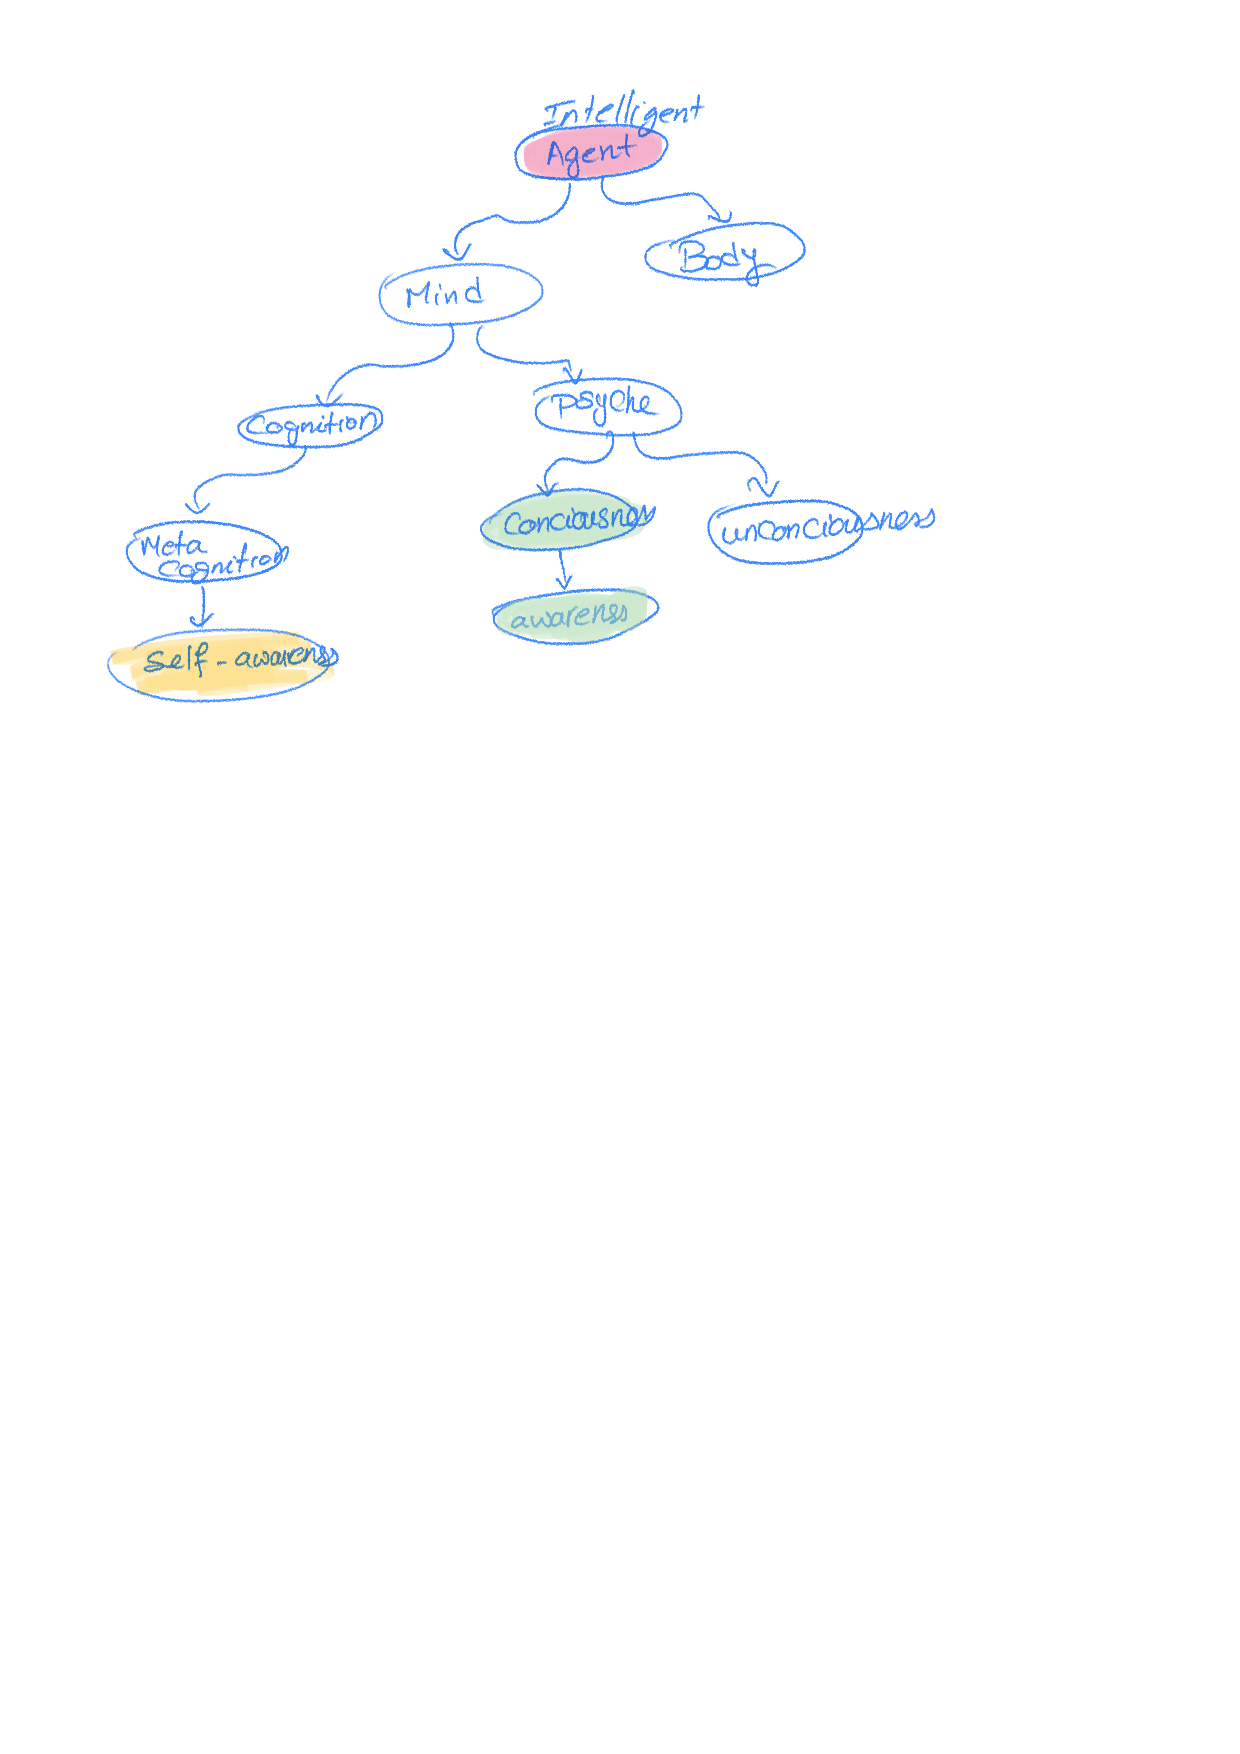
\includegraphics[width=0.9\textwidth]{self_awareness_tree.png}
   \end{figure}

   \section{Descrepency detection}
      \subsection{Novelty detection}
         Neuronal activity leads to recognizing new patterns. \href{/repo/nd_datascience_learning_project/src/machine_learning/model/discrepancy_detection/novelty/novelty.tex}{click here}
         \begin{itemize}
            \item it is neunoral
            \item previousely unseen, but potentially valid patterns
            \item It is about sensory patterns
         \end{itemize}

      \subsection{Anomaly detection}
         A data point not matching with teh rest of existing data
         \href{/repo/nd_datascience_learning_project/src/machine_learning/model/discrepancy_detection/anomaly/anomaly.tex}{see here}

      \subsection{Noise detection}
      Refers to neuronal electrical fluctuations \href{/repo/nd_datascience_learning_project/src/signal_processing/noise/noise.tex}{see here} it could be considered as a form of signal noise \href{location}{text}

      \subsection{Outlier detection}

      \subsection{The relation}
         \begin{figure}[H]
            \centering
            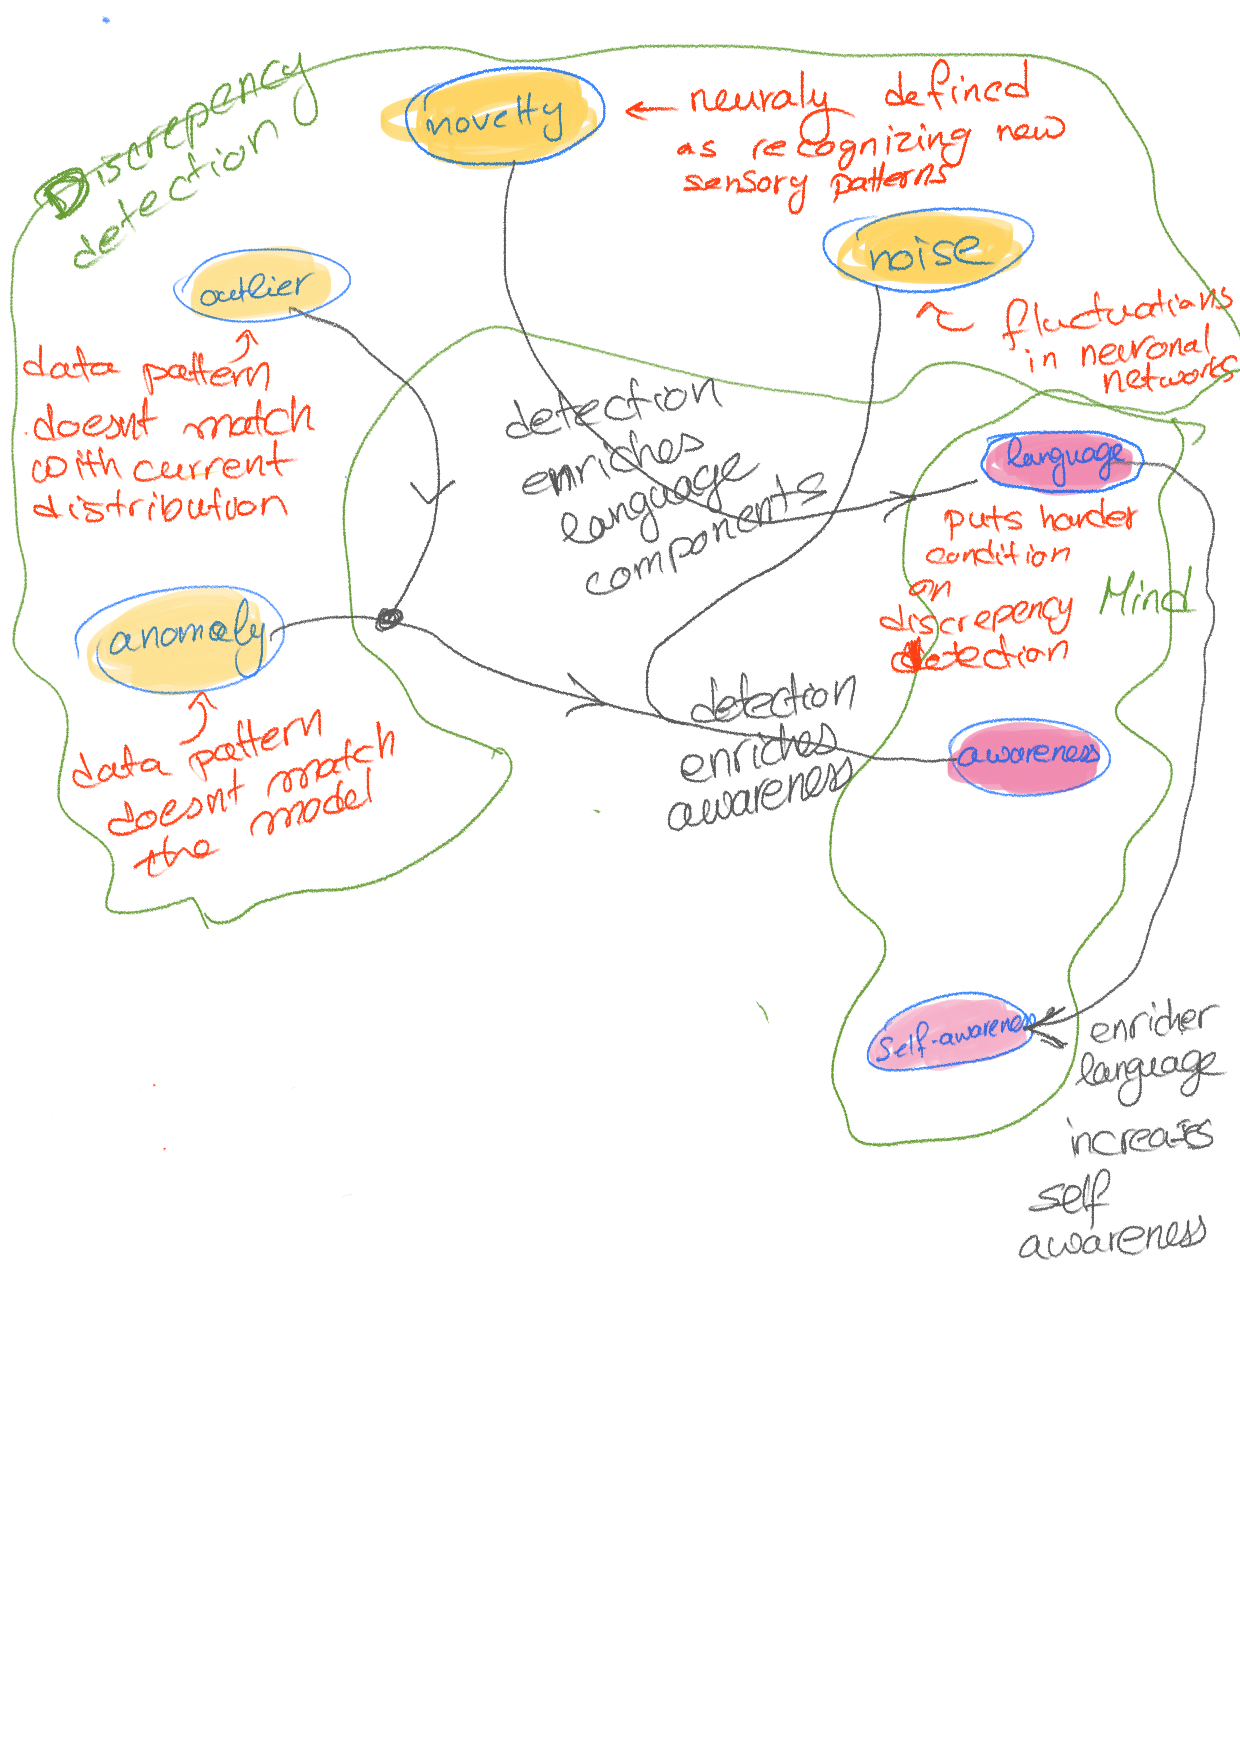
\includegraphics[width=0.9\textwidth]{novelty_detection.png}
         \end{figure}

         %    \bibliographystyle{plain}
         %    \bibliography{/home/donkarlo/Dropbox/repo/nd_shared_research/bibliography/bibliography.bib}
\end{document}